\documentclass[12pt]{article}
%\documentclass[conference]{IEEEtran}
%\usepackage[title]{appendix}
%\usepackage[T1]{fontenc}
%\usepackage[latin9]{inputenc}
\usepackage{geometry}
\geometry{verbose,tmargin=1cm,bmargin=2cm,lmargin=1cm,rmargin=1cm}
\bibliographystyle{IEEEtran}

%\setlength{\parindent}2}
\usepackage{amsmath}
\usepackage{amssymb}
\usepackage{caption}
\usepackage{adjustbox}
\usepackage{graphicx}% http://ctan.org/pkg/graphicx
\PassOptionsToPackage{normalem}{ulem}
\usepackage{ulem}
\usepackage{setspace}
\linespread{1.5}
\usepackage{algorithm}
\usepackage{enumitem}
\setlist[enumerate]{label*=\arabic*.}
\usepackage{algpseudocode}
\usepackage{hyperref}
\usepackage{listings}
\usepackage{amsmath}
\usepackage{graphicx}
\hypersetup{
	colorlinks = True,
	linkcolor = blue,
	anchorcolor = blue,
	citecolor = blue,
	filecolor = blue,
	urlcolor = blue
}
\usepackage{amsthm}
\usepackage{setspace}

% \usepackage{titlesec}
% \titleformat{\section}
%   {\normalfont\normalsize\bfseries}{\thesection.}{1em}{}
% \titleformat{\subsection}
%   {\normalfont\normalsize\itshape}{\thesubsection.}{1em}{}
% \titleformat{\subsubsection}
%   {\normalfont\normalsize\itshape}{\thesubsubsection.}{1em}{}

\newtheorem{definition}{Definition}
\newcommand{\R}{\mathbb{R}}
\renewcommand\thesubsection{\Alph{subsection}}
\makeatletter
\date{}

\makeatother

\usepackage{babel}
\begin{document}

\title{Unsupervised Electroluminescence Image Clustering for Automated Defect Detection}
  %  \date{\today} 
	
 \author{\href{mailto:bgp12@case.edu}{Benjamin G. Pierce}$^1$,
        \href{mailto:rxc542@case.edu}{Rounak Chawla}$^2$, and 
        \href{mailto:mau13@case.edu}{Maris Usis}$^3$\\
        $^1$ Department of Materials Science and Engineering\\
        $^2$ Department of Computer and Data Sciences\\
        $^3$ Department of Electrical and Computer Engineering}
\maketitle
\begin{abstract}

Photovoltaics (PV) have become an increasingly inexpensive source of renewable energy in recent years, largely due to maturing technology and economies of scale. 
As the total amount of solar PV installed exceeds 1 terawatt (as of 2022), quantification of PV performance becomes crucial to manufacturers, insurers, and system operators. 
A commonly used form of nondestructive testing of PVs is electroluminescence (EL) imaging, where a bias is applied to a PV cell or module and the usable area emits light in the near-infrared spectrum, which is captured by a sensitive camera. 
These EL images are commonly used to manually and qualitatively evaluate modules by the failures or flaws they exhibit, commonly cracking, corrosion, or various manufacturing defects. 
However, it is difficult to do this at scale, especially in an assembly line fashion. 
Previous works have explored the possibilities of using convolutional neural networks (CNNs) to automatically classify EL images, but these CNNs require labeled training data in large quantities, and are vulnerable to the imbalanced class problem. 
In this work, we introduce a unsupervised convolutional auto-encoder (CAE) model, and compare it to a classical unsupervised image processing approach. 
We will show that unsupervised approaches can attain very good accuracy scores on multiple EL image datasets without the need for costly training data with labels.
\end{abstract}

\section{Project Overview}
As the world moves towards renewable and reduced emissions energy sources, photovoltaics (PV) have become a economically dominant technology, as the price on PV modules continues to fall. 
The variable cost of fuel (sunlight) for PV is zero, but the large upfront capital expenditure of PV makes it an amortized asset, meaning that in order to be financially viable, a PV system must have a long expected lifetime. 
Defects in PV modules, introduced in manufacturing, shipping, or in the field, can significantly reduce system lifetime. 
Therefore, there is a enormous economic interest in detecting and measuring possible defects in a PV module before, during, and after its lifetime in the field. 


One measurement that is used for this purpose is electroluminescence (EL), which generates an image of the PV module that quantifies how well it can produce electricity. 
The physics behind an EL image is relatively straightforward. 
When operating, a solar panel generates electricity through the photovoltaic effect, where light provides the necessary energy for electrons in the valence band of the module material (boron or phosphorus doped silicon) to excite beyond their valence band and become free electrons, which can move across a p-n junction to induce a current. 

If this is run in reverse and a current is \textit{applied} to the PV panel, it will then \textit{emit} light in the near-infrared spectrum, but only in areas where it would have produced light in normal operation. 
This makes an EL image a valuable measurement of the module, as dark areas in the image correspond to where the module does not produce power.  
This procedure is commonly used as part of an assembly line quality assurance step, or as a field measurement to evaluate module lifetime. 
In either case, evaluation of when a EL image looks different from the ordinary is a useful step to automate, and if needed, evaluate manually. 


However, manual inspection of many EL images is quite costly, and as the PV industry continues to scale up in near short term, the industry needs methods to perform automated review of EL images. 
The literature over the last few years has been focused on using Convolutional Neural Networks (CNNs) to classify EL images based on labeled examples, as in \cite{akram_cnn_2019}. 
This methodology essentially automates the processing of selecting filters in the spacial domain by learning convolutional kernels from the data. 
However, CNNs are very dependent on data quantity and quality, and in particular are vulnerable to the imbalanced class problem, where a dataset does not contain an adequate balance of the intended targets. 
This results in a model learning a non-useful target distribution.
For example, a model trained on a dataset with 999 EL images that represent a "Good" module, and 1 that represents a "Bad" module, the model will be correct 99.9\% of the time by simply always classifying any input as "Good".
While representative of the training set, this output is not desirable. 
Unfortunately, this scenario is very common in EL image data, as manufacturing and operations and maintenance procedures are designed for a low failure rate in order to be profitable, and companies are generally reluctant to perform destructive testing on a large scale, which would be needed to construct a complete, class-balanced dataset for supervised learning. 
Additionally, failures in PV modules can be quite diverse, and difficult to classify into well-defined classes due to different module types, manufacturing processes, and varied failure triggers in the field. 
Even expert labeling of EL images is often subjective and subject to various errors. 
These issues make supervised models like CNNs less desirable for some applications. 

Unsupervised learning, in contrast, does not require labeled training data, and seeks to estimate the natural clusters in the data, which hopefully correspond to real-world classifications. 
As they are primarily data-driven, unsupervised models can avoid human bias in the labels, and identify failure types that may not be understood \textit{a priori}. 
Additionally, clustering methods can be more robust to imbalanced classes, and are often more explainable when a misclassification occurs. 
However, the main strength of unsupervised methods in this case is in exploratory data analysis and human-in-the-loop feedback. 
Oftentimes, if a model can be used to raise a flag that a certain module has some defect, it is usually inspected manually. 
The value of automated efforts such as this is to narrow the amount of samples that require human intervention, not to replace the human element entirely, while avoiding injection of bias in a labeling process and the associated increased costs of labeling. 
Therefore, in this work, we present two types of unsupervised feature extractors, one that uses classical image processing techniques and one with a deep autoencoder model. 
By comparing these techniques to each other, we will identify which techniques perform the best across various datasets and provide actionable insight and model guidelines/code for use in industry. 


\section{Problem Statement}
Can different types of degradation/failures be detected in EL images using unsupervised image processing techniques? 
In particular, can this be done without a large dataset of labeled samples, which is what the state of the art CNN models struggle with. 

Consider Deitsch \textit{et. al.} \cite{deitsch_automatic_2019}, who developed an EL image dataset of 2624 solar cells, with annotated defect regions. 
This dataset was generated via manual annotation of the ground truth defects in the EL images with the help of an expert. 
While this led to the creation of a useful open dataset, this procedure is inefficient, non-reproducible, and inaccessible to researchers without an expert. 
As such, many unannotated EL image datasets of solar cells exist, and our project aims to examine the the representative accuracy of learned defect features from these datasets in an unsupervised setting.

\section{Objectives}
We have the following objectives:
\begin{enumerate}
    \item Construct a classical image processing pipeline that preforms better then the previous
    \item Train a CAE for automated feature extraction
    \item Compare clusters between classical and CAE model
    \item Quantify performance differences across multiple datasets
\end{enumerate}
\section{Methodology}
The overarching method has the following steps:
\begin{enumerate}
    \item Compute a feature vector $v \in \R^k$ from an image $I \in \R^{m \times n}$, where $k$ is a hyper-parameter that is empirically determined. 
    \item Assemble feature vectors for all $N$ images, forming a matrix $X \in \R^{N \times k}$.
    \item Cluster on the samples, and group each image into a cluster $1...g$, where $g$ is the desired number of groups.
    \item Map each $g_i$ to a corresponding real-world, physical classification.
\end{enumerate}
Step 1 will be performed with A) Classical Image Processing, and B) Deep Learning, which are explained below.
\subsection{Classical Image Processing (Maris)}
The classical image pipeline will follow that of our previous work in \cite{pierce_identifying_2020} where an image processing \& feature extraction pipeline is constructed to perform clustering on representative vectors of EL images. 
These vectors are extracted with a customized feature detector, which will be improved upon in this paper.
A block diagram of the pipeline is shown in Figure \ref{fig:pipeline}.
\begin{figure}[h]
    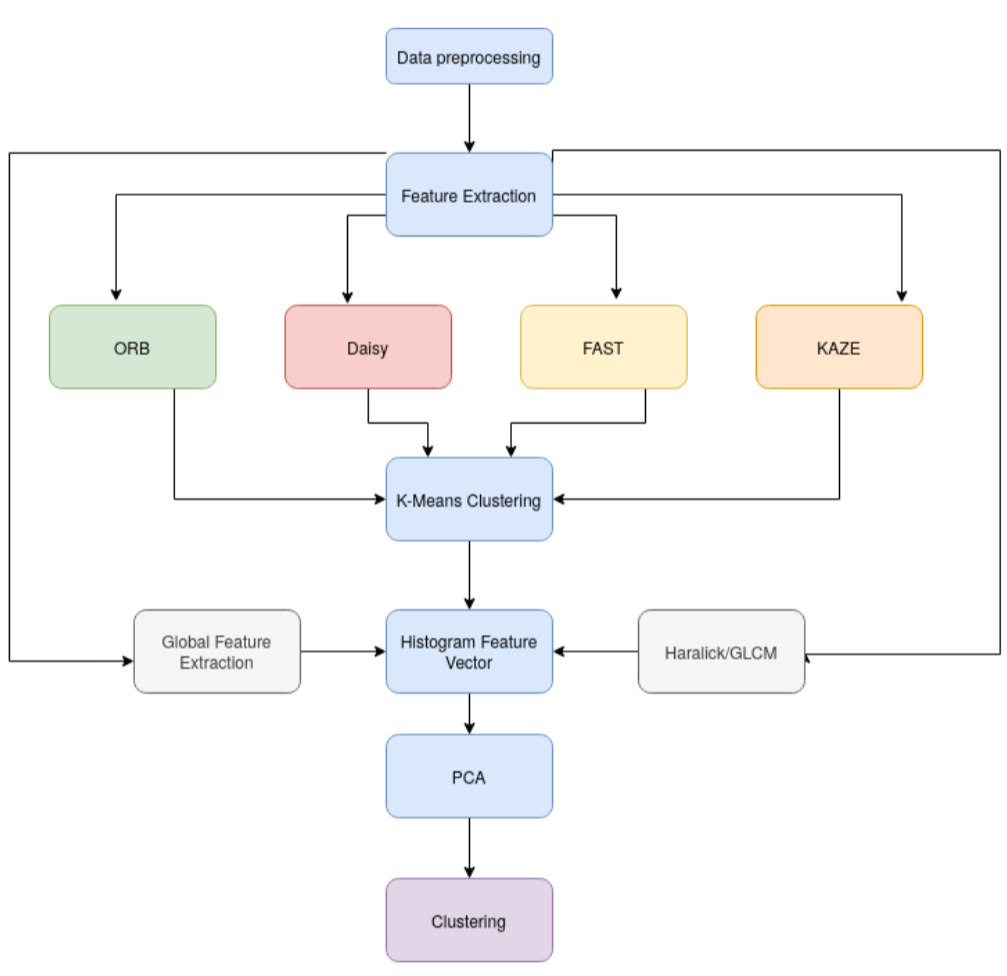
\includegraphics[width=10cm]{pipeline.png}
    \centering
    \caption{The unsupervised classical image processing framework shown in \cite{pierce_identifying_2020}. In this work, feature extractors like ORB, Daisy, FAST, and KAZE will be replaced or augmented with more current methods.}
\label{fig:pipeline}
\end{figure}

\subsection{Deep Learning (Ben)}
In this work, we will use a Convolutional Autoencoder (CAE) as the deep learning technique. 
A CAE learns many convolution kernels to automate the process of feature extraction by down-sampling a image to a vector, thereby creating a representational "bottleneck", and then up-sampling the image back up with transposed convolutions. 
The loss between the original image and reconstructed image is computed, and then backpropagated through the network to learn convolutional kernels. 

Once the model has been trained to the point where it can successfully reproduce an image, the vector "bottleneck," referred to as the latent space, is used as a vector representation of the image. 
This process can be viewed as a non-linear and high-dimensional version of Principal Component Analysis (PCA), which is commonly applied on vector data for dimensionality reduction by exploiting co-linearites in the data. 

The architecture of our model is loosely based on the U-Net design from \cite{DBLP:journals/corr/RonnebergerFB15}, and also draws concepts from the Variational Autoencoder from \cite{Subramanian2020}. 
Our full architecture is shown in detail in Figure \ref{fig:CAE}.

\begin{figure}[h]
    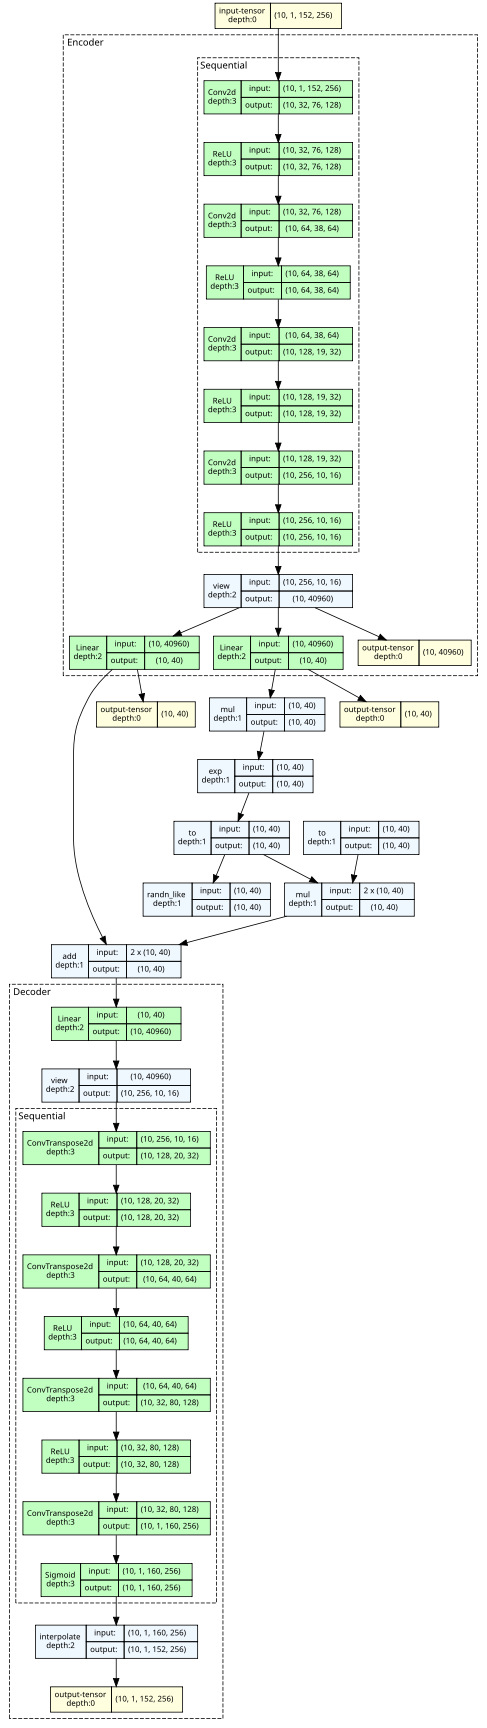
\includegraphics[width=6cm]{modelpic.png}
    \centering
    \caption{The full model architecture of our Convolutional Autoencoder, with image shapes shown for a arbitrary input.}
\label{fig:CAE}
\end{figure}

\subsection{Clustering (All)}
For both feature extraction models, we will cluster the output feature vectors using Gaussian Mixture Models (GMMs), a probabilistic clustering algorithm.
Other clustering methods, such as $k$-means, $k$-medioids, hierarchical, or density-based may also be explored, depending on model performance. 
As most are implemented using the scikit-learn Python package, they are somewhat interoperable and swappable. 

\subsection{Comparative Analysis (Rounak)}
In this step, the different models will be run and compared with each other. 
It is expected that each model will have multiple variations that have small, but signifigant differences, such as different deep learning hyperparameters, different clustering methods, and different filter coefficients. 

\section{Tools and Technologies}
This work will utilize the Python programming language. 
For the deep learning portion, the PyTorch framework will be used. 
The classical image processing pipeline will be implemented using the scikit-learn package. The individual feature extraction/segmentation algorithms will be implemented using the OpenCV framework.
Model training and hyperparameter tuning will be carried out using the CWRU HPC system, with the help of the sdlefleets package and the Singularity container environments of the SDLE Research Center. 
Finally, relevant plots and visualizations for comparative analyses will be constructed using the R programming language and the ggplot2 package. 

\section{Dataset}
There are multiple open EL image datasets available. 
The first is from CWRU, and hosted on OSF \cite{noauthor_osf_nodate}. 
Another dataset \cite{chen_automated_2022} from Lawrence Berkeley National Lab is hosted as part of the Duramat Consortium (which BGP is affiliated with), primarily focusing on crack detection. 
Deitsch \textit{et. al.}'s open EL dataset \cite{deitsch_automatic_2019} predates the former datasets, and is another benchmark in the community. 

There are also some proprietary datasets \textit{without} open data-use agreements that BGP has access to, but these will not be preferred, nor needed, likely. 

\section{Timeline}

\begin{itemize}
    \item \textbf{March 9 - March 31}: Perform further literature review and implement both sets of models (classical image processing pipeline and CAE).

    \item \textbf{April 1 - April 8}: Train models at scale and perform hyperparameter tuning, while simultaneously debugging the initial implementations.

    \item \textbf{April 9 - April 14}: Perform the comparative analysis and prepare final project report.
\end{itemize}

\section{Work Division}
Ben will be responsible for deep learning model development, dataset locating, and project direction.

Rounak will develop training schedules for each model and run them at scale with various parameters using Slurm on the CWRU HPC system. He will also compare model performance and visualize results.

Maris will implement the classical image processing pipeline.

All three of us will implement and test different clustering methods on the resultant feature vectors.

Team members are communicating via email, with periodic Zoom meetings scheduled before each milestone for progress updates.

% @rounak running models at scale on all datasets using slurm?
% @maris developing classical image processing models based on my prevoius code?

\bibliography{refs_490} % Entries are in the refs.bib file
\end{document}